\begin{figure}[t!]
\newcommand{\inlineCheck}{\,\smash{\raisebox{-.3ex}{
\includegraphics[height=2ex]{figures/wmtask/check.png}}}\,}
\newcommand{\inlineCross}{\,\smash{\raisebox{-.3ex}{
\includegraphics[height=2ex]{figures/wmtask/cross.png}}}\,}
\vspace*{-1\baselineskip}
\centering
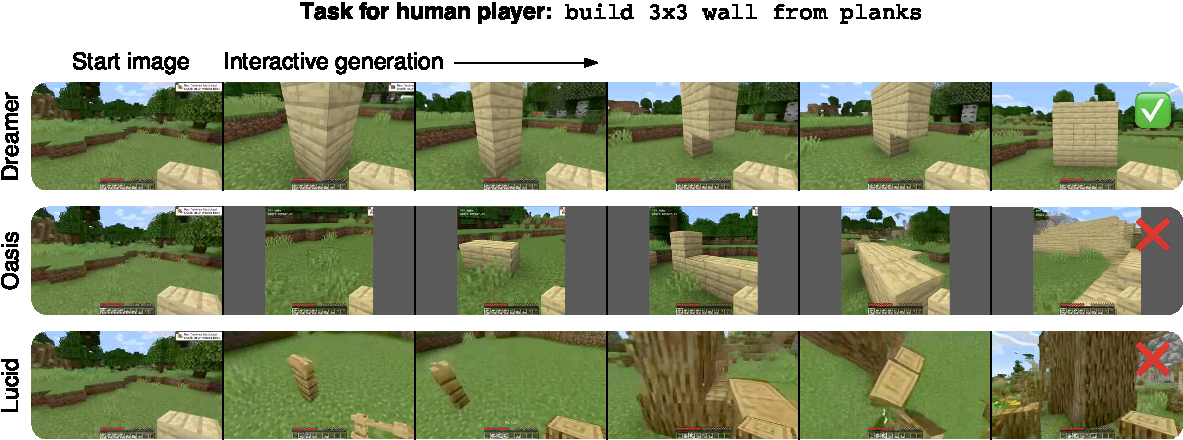
\includegraphics[width=\linewidth]{figures/wmtask/wmtask}
\caption{Human interaction. A human player counterfactually interacts with the world model in real time via mouse and keyboard to perform the same task from the same initial image.
\method is the first world model to accurately predict the object interactions and game mechanics of placing the blocks in the correct shape.
In contrast, previous Minecraft world models degrade visually, change the held item, and hallucinate structures that the player never built.
The \method world model allows the player to accomplish the task (\inlineCheck) while Oasis and Lucid do not (\inlineCross).
}
\label{fig:wmtask}
\end{figure}
